\documentclass[11pt]{article}

\usepackage[margin={1in,1in}]{geometry}
\usepackage{amssymb,amsmath}
\usepackage{subfig}
\usepackage{graphicx}
\usepackage{color}
\usepackage{listings}
\usepackage{multicol}
\usepackage{titlesec}
\usepackage{float}
\usepackage{booktabs}

\setlength{\columnsep}{20pt}
\setlength{\parindent}{0pt}

\graphicspath{{figures/}}
\newcommand{\ut}{\ensuremath{\frac{\partial u}{\partial t}}}
\newcommand{\uxx}{\ensuremath{\frac{\partial^2 u}{\partial x^2}}}
\newcommand{\Qt}{\ensuremath{\frac{dQ}{dt}} }
\renewcommand{\labelitemi}{$\vcenter{\hbox{\tiny$\bullet$}}$}
\begin{document}

\definecolor{dkgreen}{rgb}{0,0.6,0}
\definecolor{gray}{rgb}{0.5,0.5,0.5}
\definecolor{mauve}{rgb}{0.58,0,0.82}
\definecolor{red}{rgb}{0.8,0,0}

\lstset{frame=tb,
    language=Matlab,
    aboveskip=3mm,
    belowskip=3mm,
    showstringspaces=false,
    columns=flexible,
    basicstyle={\small\ttfamily},
    numbers=none,
    numberstyle=\tiny\color{gray},
    keywordstyle=\color{blue},
    commentstyle=\color{dkgreen},
    stringstyle=\color{mauve},
    breaklines=true,
    breakatwhitespace=true
    tabsize=3
}

\lstset{frame=tb,
    language=Ruby,
    aboveskip=3mm,
    belowskip=3mm,
    showstringspaces=false,
    columns=flexible,
    basicstyle={\small\ttfamily},
    numbers=none,
    numberstyle=\tiny\color{gray},
    keywordstyle=\color{blue},
    commentstyle=\color{dkgreen},
    stringstyle=\color{red},
    breaklines=true,
    breakatwhitespace=true
    tabsize=2
}

\titleformat{\section}
  {\large\scshape}{\thesection}{1.2em}{}

\titleformat{\subsection}
  {\small\scshape}{\thesubsection}{1em}{}

\begin{center}
    \vspace*{2cm}
    
    \hrule
    \vspace*{0.5cm}
    \Large
    \textbf{The Impact of ``I Like Bernie, But...'' on the Precinct Results of the Iowa Democratic Caucus}
    \vspace*{0.5cm}
    \hrule

    \vspace{0.5cm}
  
    \Large
    CS 170A -- Mathematical Modeling Methods -- Final Project

    \vspace{0.2cm}
    \textbf{Jacob Nisnevich}
    \vspace{1cm}
  
    \textbf{Abstract}\\
    \vspace{0.5cm}
    \normalsize
    \begin{minipage}{0.8\textwidth}
        Although it is difficult to assess the exact impact of the website on the outcome and precinct results of the first in the nation Democratic caucus in Iowa, correlation and linear regression analysis shows a slight positive correlation between sessions normalized by precinct population and Bernie Sanders's precinct net delegate results.
    \end{minipage}
    \vspace{0.5cm}
\end{center}

\begin{multicols}{2}

\section{Introduction}

Over the past year or so, the 2016 presidential race has gripped the nation on both the Republican and Democratic sides. With insurgent, anti-establishment candidates like Bernie Sanders and Donald Trump rising beyond expectations, this years edition of the race for the White House has been unique in many ways. \\

As is tradition, the first major test of any presidential campaign is the Iowa caucus, the first election of the primary season. Although Iowa frequently does not choose the eventual candidate correctly, the caucus has the potential to build momentum or draw much needed attention to an otherwise unlikely candidate. \\ 

Like many young voters, the presidential campaign of Bernie Sanders drew my attention immediately due to his blunt and unfiltered honesty and idealistic platform. As such, I volunteered my coding skills to help the campaign. \\

About a week prior to the Iowa democratic caucus, my brother and I launched ilikeberniebut.com to address common criticisms of Bernie Sanders with well-sourced and concise rebuttals. The response we received was completely unexpected with thousands of shares and tweets on Facebook and Twitter respectively. By the time of the Iowa caucus on February 1, our website had been viewed over 1.5 million times nationwide, including over 20,000 times in the crucial state of Iowa. \\

Although it is unlikely that the website itself had a significant impact on the outcome of the Iowa caucus, it is quite possible that viewing the site changed some minds in the crucial last few days before the election. To track the effect of the website, I have combined four different data sources: \\

\begin{enumerate}
    \item Google Analytics data for ilikeberniebut.com
    \item Iowa precinct caucus results from the Iowa Democratic party website$^1$
    \item List of Iowa cities from Wikipedia to convert Google Analytics city data to counties$^5$
    \item Iowa census data for county demographics$^2$
\end{enumerate}
 
\section{Data Acquisition}

\subsection{Google Analytics Data}

The Google Analytics data was the simplest to acquire. I simply exported the per-city session data, which reflects how many times the site was visited in each city in Iowa.

\end{multicols}

\begin{figure}[H]
    \caption{Per-City Session Data for ilikeberniebut.com in Iowa}
    \centering
    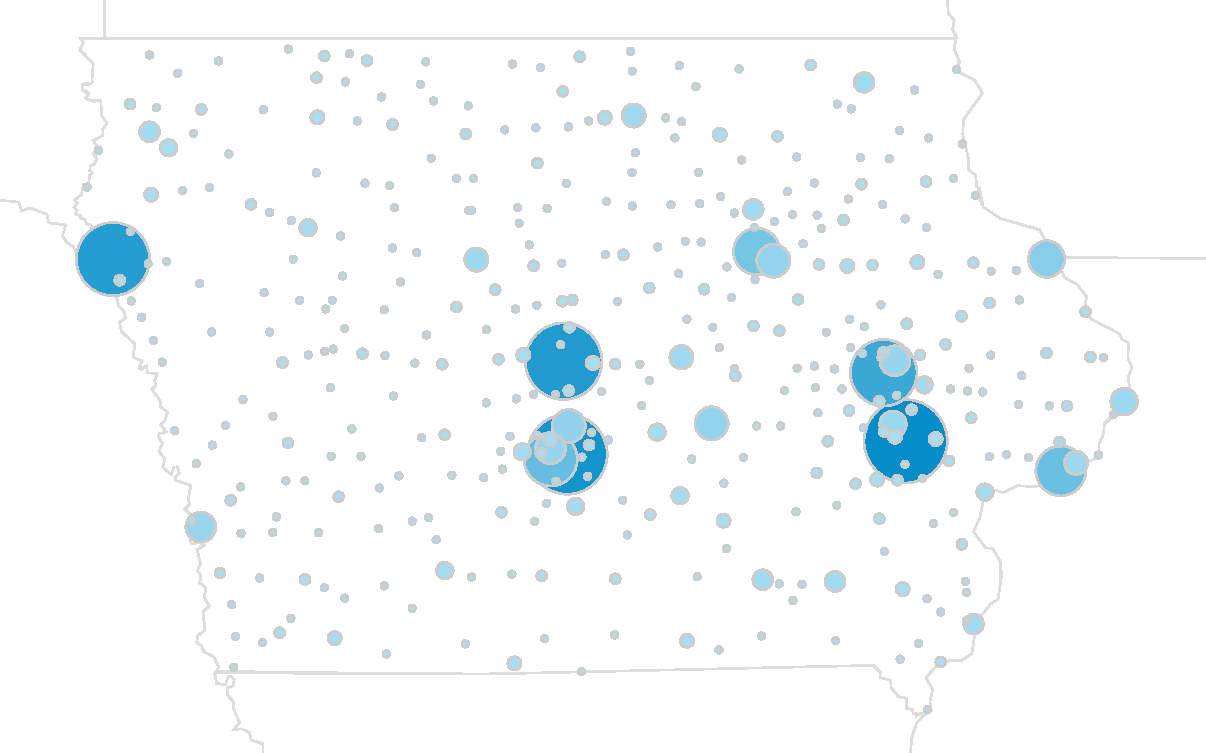
\includegraphics[width=0.9\textwidth]{google-analytics}
\end{figure}
 
\begin{multicols}{2}

The primary issue with this raw data is that as it is per-city session data, it can't be directly compared with caucus per-county results.

\subsection{Iowa Caucus Precinct Results}

The next data that was collected was the per-county precinct results for the Iowa Democratic caucus. This data was grabbed directly from the Iowa Democratic party website. Although they don't make the information freely downloadable, by setting a breakpoint in their client-side code that displays the caucus results I was able to extract the precinct data in the form of a JSON data file. \\

Using a fairly simple Ruby script (\underline{Appendix A}) I converted the JSON data to a CSV file that could more easily be transformed and analyzed in Matlab.

\subsection{Iowa Cities List from Wikipedia}

In order to be able to directly compare the per-city session data with the per-county election results, I extracted a list of Iowa cities along with the respective counties from a Wikipedia page. \\

This was done with a fairly simple HTML scraping Ruby script using the popular Nokogiri library (\underline{Appendix B}). \\

Using this list, I was able to convert the city session data to county session data with another Ruby script (\underline{Appendix C}).

\subsection{Iowa Demographics Data}

The final data that I collected for the complete dataset was demographic data for each county in Iowa from US Census data. For this particular information, I simply manually downloaded the data in the form of CSV files and added it to the overall dataset. \\

The demographics that I have included are: \textbf{Population}, \textbf{Median Age}, \textbf{Median Household Income}, \textbf{High School Graduate}, \textbf{Bachelor's Degree}, \textbf{Percent Rural}.\\  

Before finalizing the dataset, I also normalized the Google Analytics session data by county population to minimize the impact of the sheer number of people in each county on the overall website view county. \\

The full dataset can be seen in \underline{Appendix D}.

\section{Analysis}

\subsection{Correlation Analysis}

In order to get a better understanding of the relationships between a few of the variables in the large set of data, I first computed the correlation matrix of the Iowa statistics matrix. The MATLAB script used to compute this matrix can be seen in \underline{Appendix E}.

\end{multicols}

\begin{table}[H]
\centering
\caption{Correlation Matrix for Iowa Data}
\tiny
\makebox[\textwidth][c]{
\begin{tabular}{llllllllllll}
 & \textbf{Pop.} & \textbf{Age} & \textbf{MHI} & \textbf{HS Grad} & \textbf{B. Deg.} & \textbf{\% Rur.} & \textbf{Ses.} & \textbf{Ses. (Norm.)} & \textbf{Sand. Del.} & \textbf{Clin. Del.} & \textbf{Del. Diff.} \\
\textbf{Pop.} &   & -0.5368 & 0.2630  & 0.3136  & 0.5699  & -0.5935 & 0.8927  & 0.5031  & 0.9753  & 0.9853  & -0.1352 \\
\textbf{Age} & -0.5368 &   & -0.3645 & -0.2533 & -0.7035 & 0.5485  & -0.6438 & -0.7187 & -0.5681 & -0.4893 & -0.3481 \\
\textbf{MHI} & 0.2630  & -0.3645 &   & 0.4739  & 0.3608  & -0.0705 & 0.1898  & 0.1049  & 0.2681  & 0.2841  & -0.1036 \\
\textbf{HS Grad} & 0.3136  & -0.2533 & 0.4739  &   & 0.6325  & -0.2076 & 0.3878  & 0.4167  & 0.3999  & 0.3449  & 0.2424  \\
\textbf{B. Deg.} & 0.5699  & -0.7035 & 0.3608  & 0.6325  &   & -0.5109 & 0.7340  & 0.7887  & 0.6657  & 0.5628  & 0.4611  \\
\textbf{\% Rur.} & -0.5935 & 0.5485  & -0.0705 & -0.2076 & -0.5109 &   & -0.5287 & -0.5213 & -0.5639 & -0.5269 & -0.1379 \\
\textbf{Ses.} & 0.8927  & -0.6438 & 0.1898  & 0.3878  & 0.7340  & -0.5287 &   & 0.7594  & 0.9288  & 0.8808  & 0.1620  \\
\textbf{Ses. (Norm.)} & 0.5031  & -0.7187 & 0.1049  & 0.4167  & 0.7887  & -0.5213 & 0.7594  &   & 0.5698  & 0.4584  & 0.5123  \\
\textbf{Sand. Del.} & 0.9753  & -0.5681 & 0.2681  & 0.3999  & 0.6657  & -0.5639 & 0.9288  & 0.5698  &   & 0.9801  & 0.0136  \\
\textbf{Clin. Del.} & 0.9853  & -0.4893 & 0.2841  & 0.3449  & 0.5628  & -0.5269 & 0.8808  & 0.4584  & 0.9801  &   & -0.1850 \\
\textbf{Del. Diff.} & -0.1352 & -0.3481 & -0.1036 & 0.2424  & 0.4611  & -0.1379 & 0.1620  & 0.5123  & 0.0136  & -0.1850 &  
\end{tabular}
}
\end{table}

\begin{multicols}{2}

The most important result of this matrix is the correlation between delegate difference and normalized sessions of 0.5123. This indicates a positive correlation between visits to ilikeberniebut.com and the margin of a Sanders victory. While this does suggests that these two factors could be linked in some way, it is still insufficient to show a cause-and-effect relationship. \\

\subsection{Linear Regression}

To further illustrate the relationship discovered in the previous analysis, below, in \underline{Figure 2}, is a plot of Iowa counties plotted with normalized sessions on the x-axis and the delegate difference on the y-axes. In the plot, counties won by Bernie Sanders are denoted with blue dots, while counties won by Hillary Clinton are marked with red dots. \\

Also included in the plot is the linear regression line that shows the correlation between the two variables. As expected, it's slope matches the correlation of 0.5123. The code for this MATLAB script can be seen in \underline{Appendix F}.

\end{multicols}

\begin{figure}[H]
    \caption{Linear Regression for Sessions and Delegate Difference}
    \centering
    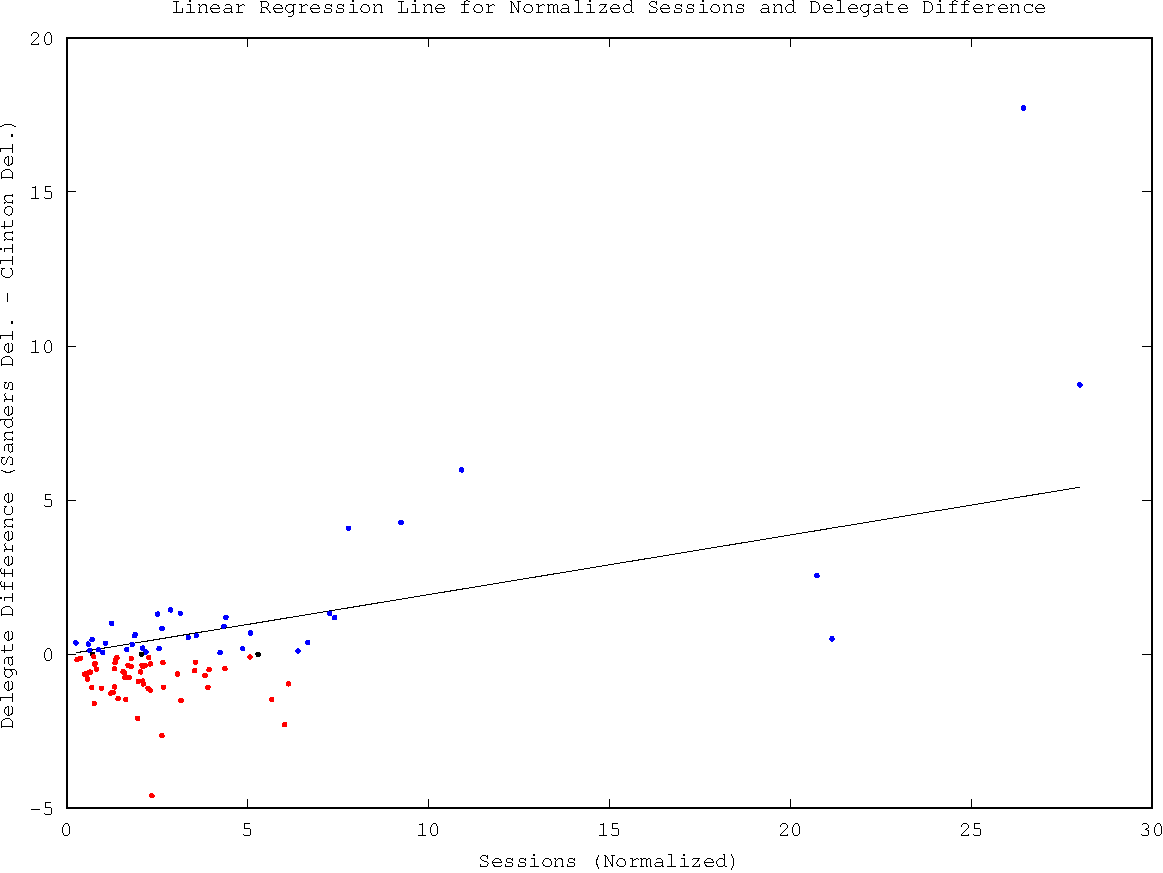
\includegraphics[width=0.9\textwidth]{iowa-corr-sessions-crop}
\end{figure}
 
\begin{multicols}{2}

\subsection{Multi-variate Linear Regression Model}

One way to show the causation relationship betweeen normalized sessions and delegate differences is by showing that a model consisting of only demographic data cannot predict the outcomes of the Iowa caucus. In order to do this, I trained a linear regression model using the county demographic data. \\

The first step to training the linear regression model was identifying the training data and the target vector. The training data was simply the matrix of demographic data for each county. Additionally, in order to prevent bias from any single demographic variable I normalized the training data columns from 0 to 1. The MATLAB code for this is shown below: \\

\begin{lstlisting}
iowaDemographics = csvread("iowa-demographics-raw.csv");

for i = 1:5
  row = iowaDemographics(:,i);
  iowaDemographics(:,i) = (row .- min(row)) ./ (max(row) - min(row));
end

csvwrite("iowa-demographics-norm.csv");
\end{lstlisting}

Using this data as a training set and the deleate difference column as the target data, I trained a multi-variable linear regression model using a Ruby implementation of the \texttt{liblinear} linear regression library. The full script used to train the model can be seen in \underline{Appendix G}. \\

With this demographics-based model in hand, I inputed the original data set and stored the resulting predictions. The predictions produced by the linear regression model are shown below in \underline{Table 2}.

\end{multicols}

\begin{table}[H]
\centering
\caption{Predicted vs Actual County Results Using a Demographics-Only Linear Model}
\small
\begin{tabular}{lllllll}
\multicolumn{1}{c}{\textbf{County}} & \multicolumn{1}{c}{\textbf{Predicted}} & \multicolumn{1}{c}{\textbf{Actual}} &  & \multicolumn{1}{c}{\textbf{Counties}} & \multicolumn{1}{c}{\textbf{Predicted}} & \multicolumn{1}{c}{\textbf{Actual}} \\ \toprule
Johnson       & 7.84      & 17.72  &  & Palo Alto  & -0.4      & -0.27  \\
Story         & 7.82      & 8.74   &  & Sac        & -0.47     & -0.3   \\
Linn          & -0.26     & 5.98   &  & Greene     & -0.07     & -0.31  \\
Black Hawk    & 0.25      & 4.27   &  & Humboldt   & 0.03      & -0.33  \\
Jefferson     & 4.57      & 4.09   &  & Adair      & -0.69     & -0.36  \\
Woodbury      & -1.1      & 2.55   &  & Emmet      & -0.83     & -0.36  \\
Muscatine     & -0.99     & 1.44   &  & Jackson    & -1.27     & -0.36  \\
Des Moines    & -0.06     & 1.33   &  & Guthrie    & -0.24     & -0.4   \\
Winneshiek    & 1.04      & 1.32   &  & Madison    & -0.68     & -0.4   \\
Boone         & 0.62      & 1.3    &  & Appanoose  & -0.32     & -0.47  \\
Marshall      & -0.53     & 1.2    &  & Wright     & -1.01     & -0.47  \\
Scott         & -0.7      & 1.19   &  & Davis      & -1.39     & -0.48  \\
Butler        & -1.52     & 1      &  & Buchanan   & -1.11     & -0.5   \\
Cedar         & 0.03      & 0.91   &  & Tama       & -0.66     & -0.53  \\
Montgomery    & -0.62     & 0.84   &  & Louisa     & -0.88     & -0.56  \\
Clinton       & -1.15     & 0.69   &  & Fayette    & -0.26     & -0.57  \\
Shelby        & 0.19      & 0.64   &  & Franklin   & -0.47     & -0.58  \\
Jones         & -0.98     & 0.6    &  & Lucas      & -1.24     & -0.6   \\
Winnebago     & 0.76      & 0.6    &  & Wayne      & 0.1       & -0.6   \\
Pottawattamie & -1.7      & 0.54   &  & Clarke     & -0.52     & -0.64  \\
Poweshiek     & 0.8       & 0.5    &  & Monona     & -0.67     & -0.64  \\
Harrison      & -1.01     & 0.47   &  & Ringgold   & 0.3       & -0.65  \\
Union         & 0.39      & 0.38   &  & Washington & -0.53     & -0.69  \\
Worth         & -0.64     & 0.37   &  & Audubon    & -1.15     & -0.75  \\
Cherokee      & 0.22      & 0.36   &  & Plymouth   & 0.08      & -0.75  \\
Lyon          & -1.2      & 0.33   &  & Taylor     & -0.34     & -0.8   \\
Howard        & -1.12     & 0.31   &  & Mahaska    & -0.06     & -0.87  \\
Grundy        & -0.24     & 0.2    &  & Hancock    & -0.01     & -0.88  \\
Cerro Gordo   & 0.8       & 0.18   &  & Bremer     & 1.05      & -0.96  \\
Dickinson     & 1.44      & 0.18   &  & Delaware   & -0.72     & -0.96  \\
Clayton       & -0.7      & 0.16   &  & Hardin     & 0.41      & -1.06  \\
Fremont       & -0.16     & 0.15   &  & Floyd      & 0.02      & -1.07  \\
Van Buren     & -0.23     & 0.13   &  & Hamilton   & 0.64      & -1.07  \\
Sioux         & 0.07      & 0.11   &  & Pocahontas & 0.24      & -1.08  \\
Clay          & 0.56      & 0.07   &  & Cass       & 0.7       & -1.1   \\
Monroe        & -0.64     & 0.05   &  & Keokuk     & -0.62     & -1.1   \\
Page          & 0.57      & 0.05   &  & Jasper     & -0.3      & -1.17  \\
Buena Vista   & 0.56      & 0      &  & Mitchell   & -0.82     & -1.25  \\
Calhoun       & 0.21      & 0      &  & Chickasaw  & -0.82     & -1.26  \\
Henry         & 0.55      & 0      &  & Benton     & -1.05     & -1.44  \\
Allamakee     & -0.58     & -0.08  &  & Kossuth    & -0.72     & -1.47  \\
Decatur       & 1.09      & -0.09  &  & Webster    & 0.19      & -1.47  \\
Mills         & -0.78     & -0.11  &  & Wapello    & -0.77     & -1.5   \\
O'Brien       & -0.62     & -0.11  &  & Lee        & -1.14     & -1.59  \\
Ida           & -0.18     & -0.13  &  & Carroll    & -0.19     & -2.08  \\
Iowa          & 0.03      & -0.14  &  & Dubuque    & -0.06     & -2.28  \\
Crawford      & -1.37     & -0.17  &  & Warren     & 0.43      & -2.64  \\
Osceola       & -0.63     & -0.18  &  & Dallas     & 0.93      & -4.59  \\
Marion        & -0.16     & -0.26  &  & Polk       & -3.74     & -15.96 \\
Adams         & -0.01     & -0.27  &  &            &           &       
\end{tabular}
\end{table}

\begin{multicols}{2}

The model correctly predicted the caucus outcome (not including the degree or margin of victory) approximately 62\% of the time. While this model does perform better than random chance, it is simply not sufficiently powerful to accurately predict county results on a regular basis. \\

Using the results of the linear model's predictions we can determine the correlation between normalized sessions and margin of over-/under-prediction. The plot with sessions on the x-axis and $\Delta$ delegate difference on the y-axis can be seen below in \underline{Figure 3}.\\

\end{multicols}

\begin{figure}[H]
    \caption{Relationship between Predictions and Normalized Sessions}
    \centering
    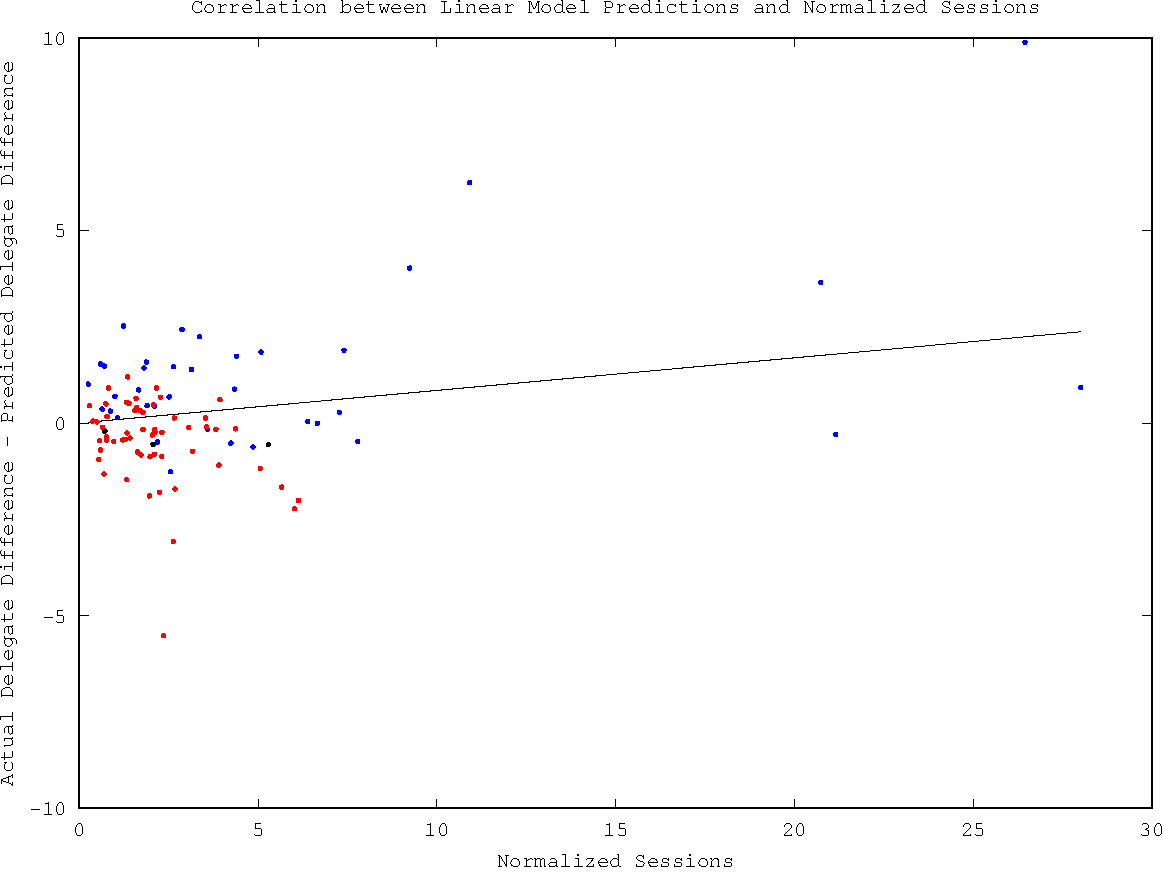
\includegraphics[width=0.9\textwidth]{iowa-corr-predictions-crop}
\end{figure}
 
\begin{multicols}{2}

Once again, Sanders counties are colored in blue and Clinton counties are colored in red. Something immediately noticeable is the fact that red and blue dots are clearly split roughly along the line $y = 0$, which would be expected from an accurate model. It is also clear that there is a slightly positive relationship between normalized sessions and $\Delta$ delegate difference. This would indicate that the model under-predicts when normalized sessions in the county are higher. While this relationship does indicate some degree of causation, the correlation coefficient was computed to be only 0.2704, which does not suggest a particularly high correlation. The MATLAB code for creating the plot and computing the correlation coefficient can be seen in \underline{Appendix H}.\\

\subsection{Principal Component Analysis}

Another method of data analysis I conducted on the county data was principal component analysis. The Iowa county data was the perfect candidate for PCA largely due to the huge amount of variables and dimensions in the dataset. Principal component analysis esssentially allowed me to identify the variables and factors that contributed most to the spread in the data. \\

\end{multicols}

\begin{table}[H]
\centering
\caption{Principal Compoments for Iowa County Data}
\begin{tabular}{lrrllrr}
\multicolumn{3}{c}{\textbf{Covariance principal components}} &  & \multicolumn{3}{c}{\textbf{Correlation principal components}} \\
\cmidrule(r){1-3} \cmidrule(r){5-7}
 & \multicolumn{1}{c}{\textbf{$e_1$}} & \multicolumn{1}{c}{\textbf{$e_2$}} &  &  & \multicolumn{1}{c}{\textbf{$e_1$}} & \multicolumn{1}{c}{\textbf{$e_2$}} \\
\midrule
Population & \underline{-0.999384} & -0.032907 &  & Population & \underline{-0.357288} & -0.328185 \\
Median Age & 0.000032 & -0.000114 &  & Median Age & \underline{0.309089} & -0.205657 \\
Median Household Income & -0.032973 & \underline{0.999442} &  & Median Household Income & -0.146486 & -0.039481 \\
High School Graduate & 0.000000 & 0.000002 &  & High School Graduate & -0.216449 & 0.198048 \\
Bachelor's Degree & -0.000001 & 0.000002 &  & Bachelor's Degree & \underline{-0.345551} & 0.276871 \\
Percent Rural & 0.000003 & 0.000004 &  & Percent Rural & \underline{0.271444} & 0.002240 \\
Sessions & -0.012011 & -0.005672 &  & Sessions & \underline{-0.379266} & -0.080844 \\
Sessions (Normalized) & -0.000052 & -0.000026 &  & Sessions (Normalized) & \underline{-0.318665} & 0.330256 \\
Sanders Delegates & -0.000296 & 0.000021 &  & Sanders Delegates & \underline{-0.373826} & -0.231996 \\
Clinton Delegates & -0.000304 & 0.000057 &  & Clinton Delegates & \underline{-0.349620} & -0.358747 \\
Delegate Difference & 0.000008 & -0.000036 &  & Delegate Difference & -0.089685 & \underline{0.659113}
\end{tabular}
\end{table}

\begin{multicols}{2}

\end{multicols}

\begin{figure}[H]
    \caption{Covariance Principal Component Analysis}
    \centering
    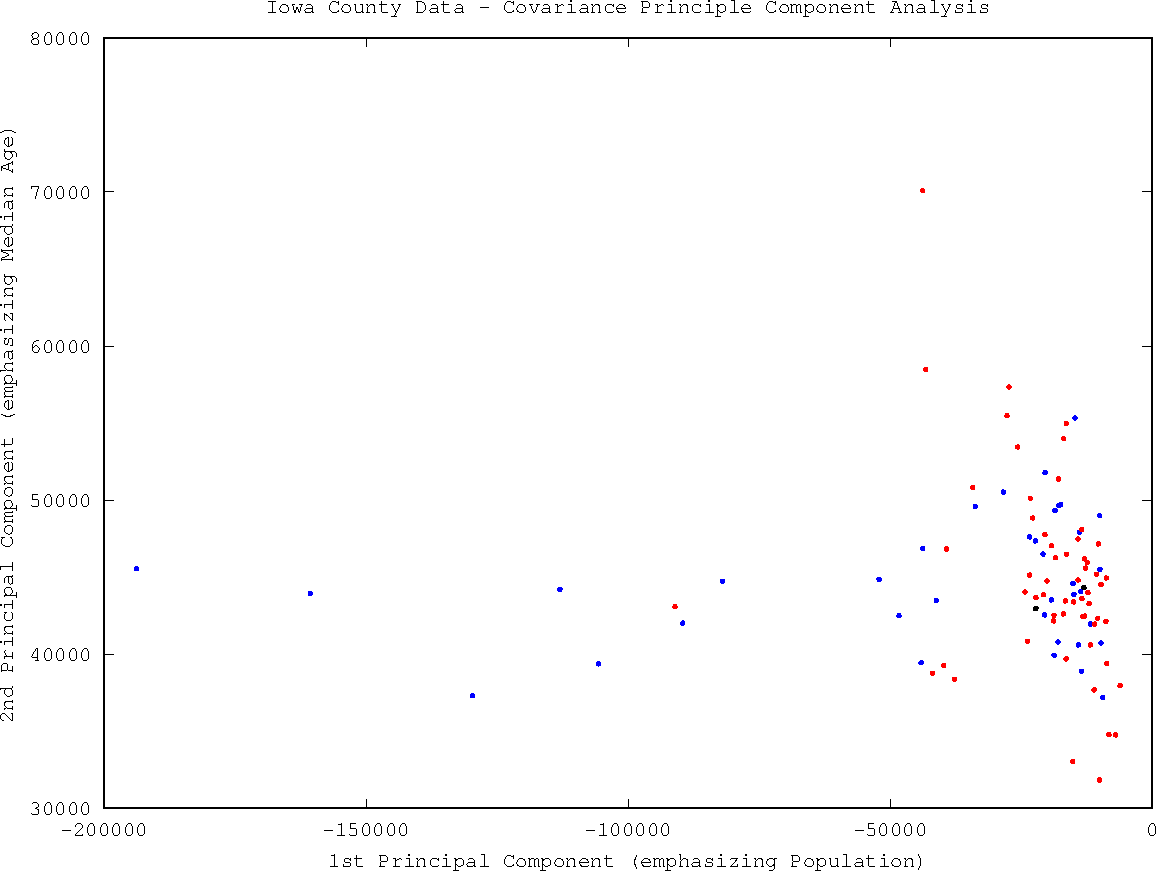
\includegraphics[width=0.9\textwidth]{iowa-cov-pca-crop}
\end{figure}
 
\begin{multicols}{2}

\end{multicols}

\begin{figure}[H]
    \caption{Correlation Principal Component Analysis}
    \centering
    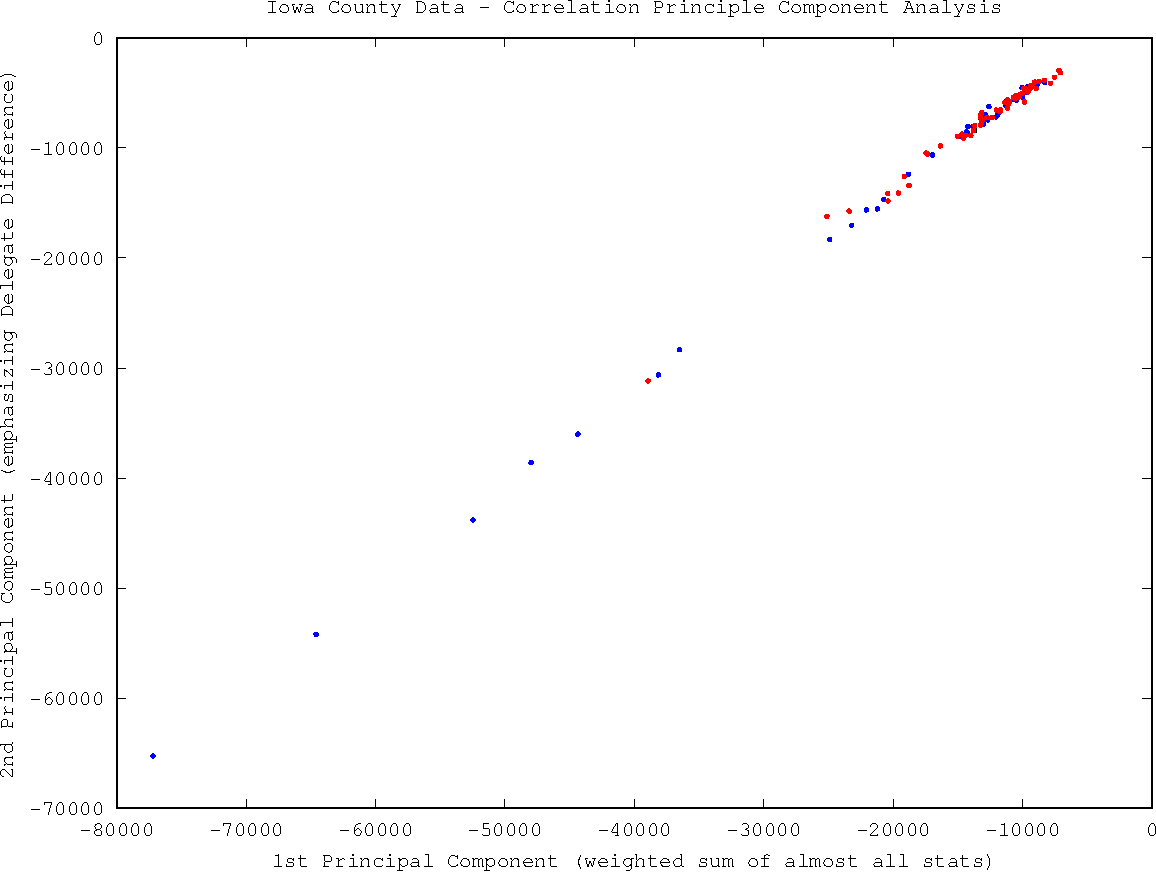
\includegraphics[width=0.9\textwidth]{iowa-corr-pca-crop}
\end{figure}
 
\begin{multicols}{2}

In \underline{Table 3}, I have displayed the resulting principal components of both the covariance and correlation matrices. For the sake of comparison, I have also included the plots for both of these principal component analyses in \underline{Figure 3} and \underline{Figure 4}. The code for computing and displaying the components and resulting plots can be found in \underline{Appendix I} and \underline{Appendix J}. \\

The first notable point given by the data is that the covariance PCA does not suit the data due to the high variance in the scales of each of the dimensions in the dataset. Note that the covariance PCA emphasizes primarily the \textbf{Population} and \textbf{Median Household Income} variables, which have by far the statistics of all the dimensions. These two variables go up to hundreds or tens of thousands while the others rarely exceed a hundred. As such, the correlation PCA is far more appropriate as it inherently scales and normalizes the dataset columns from --1 to +1. \\

On the other hand, the principal component analysis resulting from the correlation matrix emphasizes the \textbf{Delegate Difference} variable which understandably explains the spread. \\

\subsection{Miscellaneous Demographic Analysis}

One of the most interesting aspects of the Democratic race for the presidential nomination has been the distinct demographic split between supporters of Bernie Sanders and Hillary Clinton. Bernie Sanders has tended to attract young, white, liberal, and college-educated voters, while Hillary Clinton's voter base consists of older, minority, and more moderate Democratic voters. The split between the bases of the two Democratic candidates has been so clear that many political commenters and analysts such as Nate Silver have begun to utilize demographic-based models almost as much as poll-based models to predict primary election results.$^4$ \\

While I attempted to make a demographic-based linear regression model to predict county caucus results, my data lacks several crucial aspects such as race-based demographic data, which was difficult to find for each county in Iowa. Regardless, there are many interesting relationships between the performance of Bernie Sanders and demographics in the dataset. \\

Looking back to the correlation matrix for the dataset I constructed at the start of the analysis, the two demographic variables most clearly correlated with the \textbf{Delegate Difference} variable are \textbf{Median Age} and \textbf{Bachelor Degree Percentage}. The plot of median age against delegate difference can be seen below in \underline{Figure 6} with the code for the graph in \underline{Appendix K}.

\end{multicols}

\begin{figure}[H]
    \caption{Correlation between Median Age and Delegate Difference}
    \centering
    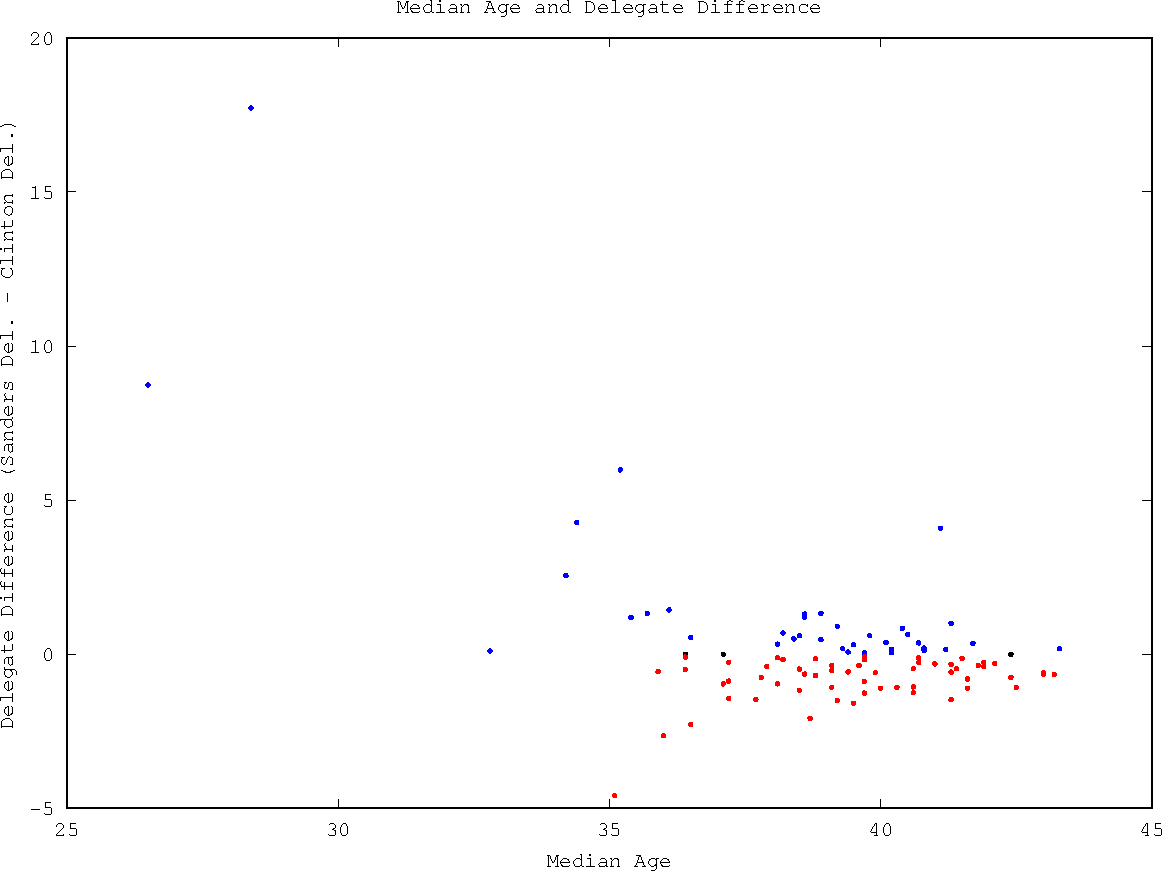
\includegraphics[width=0.9\textwidth]{iowa-corr-age-crop}
\end{figure}

\begin{multicols}{2}

As expected, as voters get older, Bernie Sanders performs significantly worse. Not surprisingly, young voters have made up a significant portion of Bernie Sanders's base. Unfortunately for Sanders however, young voters have historically failed to turnout in large numbers.$^3$ The next important demographic correlation in the data is between the percentage of Bachelor's degree recipients and the delegate difference. The plot of this data is below in \underline{Figure 7} with the MATLAB code in \underline{Appendix L}.

\end{multicols}

\begin{figure}[H]
    \caption{Correlation between Bachelor's Degree Recipients and Delegate Difference}
    \centering
    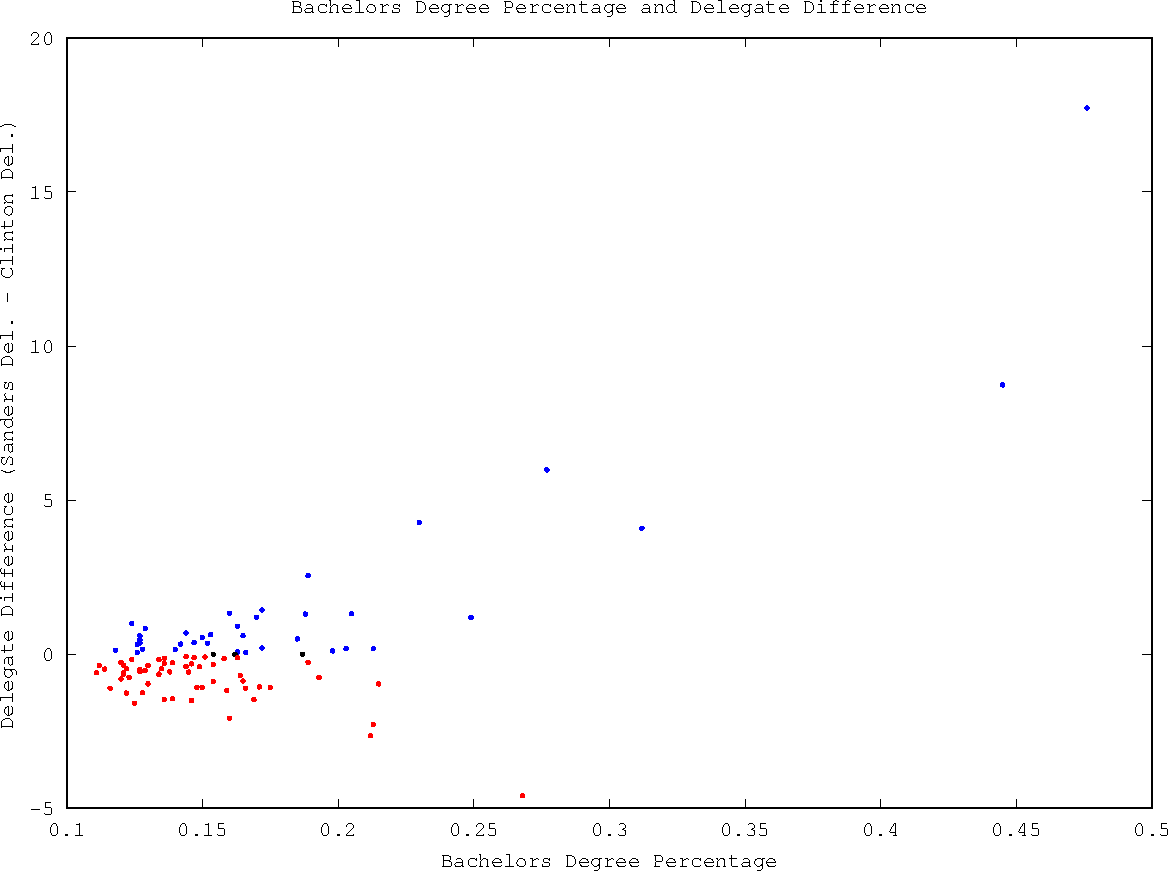
\includegraphics[width=0.9\textwidth]{iowa-corr-bach-crop}
\end{figure}

\begin{multicols}{2}

Again, as expected, Bernie Sanders performs well in counties with many college-educated voters, with him winning all counties where more than 25\% of voting age adults have Bachelor's degrees. \\

\section{Conclusion}

Through various mathematical models and analyses, I have shown that clear patterns and correlations exist when it comes to where in Iowa Bernie Sanders performed well and where he performed poorly. Furthermore, I have shown that there is in fact a positive correlation between normalized ilikeberniebut.com sessions and Iowa county delegate difference (Bernie Sanders delegates -- Hillary Clinton delegates). \\

Once this correlation was established, I attempted to show that this link was in fact a causal relationship; that viewing the website caused not-insignificant improvements in Bernie Sanders's performance in Iowa county caucus results. To do this, I created and trained a linear regression model based entirely on the demographic data I had available using the following variables:

\begin{itemize}
    \item Population 
    \item Median Age 
    \item Median Household Income
    \item High School Graduate Percent
    \item Bachelor's Degree Percent
    \item Percent Rural
\end{itemize}

While the model I created succcessfully predicted a majority of the precinct outcomes based on demographic data, it consistently underpredicted in counties where normalized sessions were relatively high. This indicated that viewing the website did have a real impact on precinct caucus results and that the demographic-only model was insufficient at predicting such results. \\

Despite the fact that all correlations do point to the fact that ilikeberniebut.com did have an impact on the outcomes of Iowa county caucuses, none of the correlation coefficients are particularly high, meaning that it is difficult to come to a decisive statistical conclusion about the data. \\

In addition to finding the real impact of ilikeberniebut.com on the Iowa caucus, my analysis confirmed and reaffirmed some of the known demographic patterns in Bernie Sanders's Democratic primary voter base, particularly with regard to age and education. \\

Although the analysis was fairly successful, there are quite a few flaws in the approach I took. The first of these flaws is my use of the delegate difference statistic as the primary measure of performance in each county. While this statistic works well for counties that are similarly sized, it fails when county populations have high variation. This is due to the fact that the margin of delegate difference could be far higher when counties have higher populations, and therefore higher delegate counts. This is reflected in the data with the most populous counties being on either end of the delegate difference spread. In retrospect, percent delegate difference would be a more reliable and consistent measure of county performance for each candidate. \\

The website, ilikeberniebut.com, certainly had some impact on caucus outcomes in certain counties, although the significance of this impact is difficult to quantify with the limited at hand.

\end{multicols}
\newpage

\setcounter{section}{0}
\renewcommand{\thesection}{\underline{Appendix \Alph{section}}}

\section{Ruby: Precinct Data to CSV}
\lstinputlisting[language=Ruby]{precinct-data-to-csv.rb}
\newpage

\section{Ruby: Get Iowa Cities}
\lstinputlisting[language=Ruby]{get-iowa-cities.rb}
\newpage

\section{Ruby: Cities to Counties}
\lstinputlisting[language=Ruby]{cities-to-counties.rb}
\newpage

\newgeometry{margin=0.5cm}
\section{Complete Dataset}
\begin{table}[H]

\centering
\tiny
\begin{tabular}{llllllllllll}
\multicolumn{1}{c}{\textbf{County}} & \multicolumn{1}{c}{\textbf{Pop.}} & \multicolumn{1}{c}{\textbf{Age}} & \multicolumn{1}{c}{\textbf{MHI}} & \multicolumn{1}{c}{\textbf{HS Grad}} & \multicolumn{1}{c}{\textbf{Bach. D.}} & \multicolumn{1}{c}{\textbf{\% Rur.}} & \multicolumn{1}{c}{\textbf{Ses.}} & \multicolumn{1}{c}{\textbf{Ses. (Norm.)}} & \multicolumn{1}{c}{\textbf{Sand. Del.}} & \multicolumn{1}{c}{\textbf{Clin. Del.}} & \multicolumn{1}{c}{\textbf{Del. Diff.}} \\ \toprule
\textbf{Adair} & 8243 & 41.8 & 47553 & 0.878 & 0.112 & 1 & 14 & 1.698410773 & 1.32 & 1.68 & -0.36 \\
\textbf{Adams} & 4482 & 41.9 & 38191 & 0.845 & 0.12 & 1 & 6 & 1.338688086 & 0.87 & 1.13 & -0.27 \\
\textbf{Allamakee} & 14675 & 39.7 & 44119 & 0.814 & 0.144 & 0.74 & 11 & 0.7495741056 & 2.96 & 3.04 & -0.08 \\
\textbf{Appanoose} & 13721 & 40.6 & 33663 & 0.814 & 0.122 & 0.58 & 60 & 4.372859121 & 2.27 & 2.73 & -0.47 \\
\textbf{Audubon} & 6830 & 42.4 & 45280 & 0.825 & 0.123 & 0.67 & 11 & 1.610541728 & 1.13 & 1.88 & -0.75 \\
\textbf{Benton} & 25308 & 37.2 & 56592 & 0.878 & 0.139 & 0.66 & 36 & 1.422475107 & 5.28 & 6.72 & -1.44 \\
\textbf{Black Hawk} & 128012 & 34.4 & 42753 & 0.865 & 0.23 & 0.13 & 1183 & 9.241321126 & 36.47 & 32.20 & 4.27 \\
\textbf{Boone} & 26224 & 38.6 & 51678 & 0.89 & 0.188 & 0.52 & 66 & 2.516778523 & 7.15 & 5.85 & 1.30 \\
\textbf{Bremer} & 23325 & 38.1 & 54482 & 0.877 & 0.215 & 0.66 & 143 & 6.130760986 & 5.44 & 6.40 & -0.96 \\
\textbf{Buchanan} & 21093 & 36.4 & 51052 & 0.846 & 0.127 & 0.72 & 83 & 3.934954724 & 4.75 & 5.25 & -0.50 \\
\textbf{Buena Vista} & 20411 & 36.4 & 43864 & 0.813 & 0.187 & 0.58 & 108 & 5.291264514 & 2.91 & 2.91 & 0.00 \\
\textbf{Butler} & 15305 & 41.3 & 50400 & 0.822 & 0.124 & 1 & 19 & 1.241424371 & 3.50 & 2.50 & 1.00 \\
\textbf{Calhoun} & 11115 & 42.4 & 44833 & 0.854 & 0.154 & 1 & 8 & 0.7197480882 & 2.00 & 2.00 & 0.00 \\
\textbf{Carroll} & 21421 & 38.7 & 46086 & 0.837 & 0.16 & 0.58 & 42 & 1.960692778 & 2.96 & 5.04 & -2.08 \\
\textbf{Cass} & 14684 & 41.6 & 40358 & 0.859 & 0.166 & 0.54 & 33 & 2.247344048 & 1.90 & 3.00 & -1.10 \\
\textbf{Cedar} & 18187 & 39.2 & 52600 & 0.877 & 0.163 & 0.84 & 79 & 4.343762028 & 4.46 & 3.54 & 0.91 \\
\textbf{Cerro Gordo} & 46447 & 39.3 & 44494 & 0.873 & 0.203 & 0.22 & 226 & 4.865760975 & 11.09 & 10.91 & 0.18 \\
\textbf{Cherokee} & 13035 & 41.7 & 44474 & 0.875 & 0.152 & 0.57 & 14 & 1.074031454 & 2.18 & 1.82 & 0.36 \\
\textbf{Chickasaw} & 13095 & 39.7 & 43990 & 0.834 & 0.122 & 0.74 & 16 & 1.221840397 & 2.34 & 3.60 & -1.26 \\
\textbf{Clarke} & 9133 & 38.6 & 42384 & 0.844 & 0.121 & 0.56 & 28 & 3.065805321 & 1.68 & 2.32 & -0.64 \\
\textbf{Clay} & 17372 & 39.4 & 44294 & 0.88 & 0.163 & 0.4 & 38 & 2.187428045 & 3.04 & 2.96 & 0.07 \\
\textbf{Clayton} & 18678 & 40.2 & 43387 & 0.826 & 0.128 & 1 & 31 & 1.659706607 & 4.08 & 3.92 & 0.16 \\
\textbf{Clinton} & 50149 & 38.2 & 47020 & 0.856 & 0.144 & 0.26 & 255 & 5.084847155 & 12.34 & 11.66 & 0.69 \\
\textbf{Crawford} & 16942 & 38.2 & 42916 & 0.785 & 0.124 & 0.65 & 23 & 1.357572896 & 2.08 & 2.25 & -0.17 \\
\textbf{Dallas} & 40750 & 35.1 & 71854 & 0.895 & 0.268 & 0.66 & 96 & 2.355828221 & 12.08 & 16.68 & -4.59 \\
\textbf{Davis} & 8541 & 38.5 & 42741 & 0.789 & 0.114 & 0.69 & 7 & 0.819576162 & 1.26 & 1.74 & -0.48 \\
\textbf{Decatur} & 8689 & 36.4 & 32242 & 0.817 & 0.151 & 0.72 & 44 & 5.063873864 & 1.41 & 1.50 & -0.09 \\
\textbf{Delaware} & 18404 & 37.1 & 48574 & 0.851 & 0.13 & 0.74 & 39 & 2.119104542 & 3.44 & 4.40 & -0.96 \\
\textbf{Des Moines} & 42351 & 38.9 & 41273 & 0.858 & 0.16 & 0.29 & 133 & 3.140421714 & 10.67 & 9.33 & 1.33 \\
\textbf{Dickinson} & 16424 & 43.3 & 50069 & 0.892 & 0.213 & 0.75 & 42 & 2.557233317 & 3.59 & 3.41 & 0.18 \\
\textbf{Dubuque} & 89143 & 36.5 & 46894 & 0.852 & 0.213 & 0.26 & 537 & 6.024028808 & 22.77 & 25.04 & -2.28 \\
\textbf{Emmet} & 11027 & 39.6 & 42979 & 0.822 & 0.13 & 0.44 & 23 & 2.085789426 & 1.32 & 1.68 & -0.36 \\
\textbf{Fayette} & 22008 & 39.4 & 41809 & 0.848 & 0.138 & 0.59 & 45 & 2.044711014 & 4.69 & 5.26 & -0.57 \\
\textbf{Floyd} & 16900 & 40.3 & 43288 & 0.859 & 0.148 & 0.55 & 66 & 3.905325444 & 3.47 & 4.53 & -1.07 \\
\textbf{Franklin} & 10704 & 41.3 & 46082 & 0.84 & 0.145 & 0.64 & 7 & 0.653961136 & 1.69 & 2.27 & -0.58 \\
\textbf{Fremont} & 8010 & 41.2 & 45897 & 0.85 & 0.14 & 1 & 7 & 0.8739076155 & 1.35 & 1.20 & 0.15 \\
\textbf{Greene} & 10366 & 41 & 44476 & 0.856 & 0.146 & 0.6 & 24 & 2.315261432 & 1.85 & 2.15 & -0.31 \\
\textbf{Grundy} & 12369 & 40.8 & 55901 & 0.865 & 0.172 & 0.8 & 26 & 2.102029267 & 2.07 & 1.87 & 0.20 \\
\textbf{Guthrie} & 11353 & 41.9 & 48626 & 0.854 & 0.149 & 1 & 24 & 2.113978684 & 1.80 & 2.20 & -0.40 \\
\textbf{Hamilton} & 16438 & 39.1 & 46994 & 0.873 & 0.175 & 0.52 & 44 & 2.676724662 & 2.47 & 3.53 & -1.07 \\
\textbf{Hancock} & 12100 & 39.7 & 48040 & 0.858 & 0.154 & 0.76 & 24 & 1.983471074 & 1.52 & 2.40 & -0.88 \\
\textbf{Hardin} & 18812 & 40.6 & 44705 & 0.857 & 0.171 & 0.58 & 25 & 1.328938975 & 2.97 & 4.03 & -1.06 \\
\textbf{Harrison} & 15666 & 38.9 & 50368 & 0.85 & 0.127 & 0.81 & 11 & 0.7021575386 & 2.73 & 2.27 & 0.47 \\
\textbf{Henry} & 20336 & 37.1 & 43887 & 0.861 & 0.162 & 0.61 & 42 & 2.065302911 & 3.50 & 3.50 & 0.00 \\
\textbf{Howard} & 9932 & 39.5 & 42421 & 0.793 & 0.126 & 0.65 & 18 & 1.812323802 & 2.15 & 1.85 & 0.31 \\
\textbf{Humboldt} & 10381 & 41.3 & 46437 & 0.863 & 0.154 & 0.61 & 8 & 0.7706386668 & 1.33 & 1.67 & -0.33 \\
\textbf{Ida} & 7837 & 41.5 & 44892 & 0.85 & 0.136 & 1 & 3 & 0.3827995406 & 0.93 & 1.07 & -0.13 \\
\textbf{Iowa} & 15671 & 38.8 & 52079 & 0.87 & 0.158 & 1 & 28 & 1.786739838 & 3.43 & 3.57 & -0.14 \\
\textbf{Jackson} & 20296 & 39.1 & 44567 & 0.815 & 0.121 & 0.72 & 44 & 2.16791486 & 4.14 & 4.50 & -0.36 \\
\textbf{Jasper} & 37213 & 38.5 & 48439 & 0.868 & 0.159 & 0.58 & 86 & 2.311020342 & 8.10 & 9.27 & -1.17 \\
\textbf{Jefferson} & 16181 & 41.1 & 41523 & 0.881 & 0.312 & 0.42 & 126 & 7.786910574 & 6.55 & 2.45 & 4.09 \\
\textbf{Johnson} & 111006 & 28.4 & 48955 & 0.937 & 0.476 & 0.27 & 2936 & 26.44902077 & 54.73 & 37.01 & 17.72 \\
\textbf{Jones} & 20221 & 38.5 & 48254 & 0.853 & 0.127 & 0.58 & 38 & 1.879234459 & 4.80 & 4.20 & 0.60 \\
\textbf{Keokuk} & 11400 & 40 & 42969 & 0.84 & 0.116 & 1 & 11 & 0.9649122807 & 1.40 & 2.50 & -1.10 \\
\textbf{Kossuth} & 17163 & 41.3 & 47812 & 0.856 & 0.136 & 0.71 & 28 & 1.631416419 & 2.13 & 3.60 & -1.47 \\
\textbf{Lee} & 38052 & 39.5 & 40921 & 0.836 & 0.125 & 0.37 & 29 & 0.7621150005 & 7.71 & 9.29 & -1.59 \\
\textbf{Linn} & 191701 & 35.2 & 53700 & 0.906 & 0.277 & 0.18 & 2093 & 10.91804425 & 63.31 & 57.33 & 5.98 \\
\textbf{Louisa} & 12183 & 35.9 & 45367 & 0.797 & 0.127 & 1 & 19 & 1.559550193 & 1.68 & 2.24 & -0.56 \\
\textbf{Lucas} & 9422 & 39.9 & 38122 & 0.791 & 0.111 & 0.52 & 15 & 1.59201868 & 1.20 & 1.80 & -0.60 \\
\textbf{Lyon} & 11763 & 38.1 & 48467 & 0.787 & 0.142 & 0.79 & 7 & 0.5950862875 & 1.13 & 0.80 & 0.33 \\
\textbf{Madison} & 14019 & 37.9 & 55607 & 0.876 & 0.144 & 0.68 & 25 & 1.783294101 & 2.80 & 3.20 & -0.40 \\
\textbf{Mahaska} & 22335 & 37.2 & 45021 & 0.826 & 0.165 & 0.52 & 47 & 2.104320573 & 3.07 & 3.93 & -0.87 \\
\textbf{Marion} & 32052 & 37.2 & 52221 & 0.84 & 0.189 & 0.44 & 114 & 3.556720329 & 6.24 & 6.50 & -0.26 \\
\textbf{Marshall} & 39311 & 38.6 & 45190 & 0.823 & 0.17 & 0.35 & 173 & 4.400803846 & 9.60 & 8.40 & 1.20 \\
\textbf{Mills} & 14547 & 38.1 & 54646 & 0.832 & 0.163 & 0.61 & 33 & 2.268508971 & 2.44 & 2.56 & -0.11 \\
\textbf{Mitchell} & 10874 & 40.6 & 46684 & 0.844 & 0.128 & 0.7 & 14 & 1.28747471 & 1.35 & 2.60 & -1.25 \\
\textbf{Monona} & 10020 & 43 & 41072 & 0.817 & 0.134 & 0.72 & 5 & 0.499001996 & 1.16 & 1.80 & -0.64 \\
\textbf{Monroe} & 8016 & 39.7 & 41103 & 0.822 & 0.126 & 0.55 & 8 & 0.998003992 & 1.34 & 1.29 & 0.05 \\
\textbf{Montgomery} & 11771 & 40.4 & 39430 & 0.818 & 0.129 & 0.49 & 31 & 2.633591029 & 1.92 & 1.08 & 0.84 \\
\textbf{Muscatine} & 41722 & 36.1 & 48671 & 0.803 & 0.172 & 0.29 & 120 & 2.876180432 & 9.72 & 8.28 & 1.44 \\
\textbf{O'Brien} & 15102 & 40.7 & 43292 & 0.807 & 0.147 & 0.71 & 21 & 1.390544299 & 1.42 & 1.53 & -0.11 \\
\textbf{Osceola} & 7003 & 39.7 & 42469 & 0.811 & 0.134 & 0.64 & 2 & 0.2855918892 & 0.38 & 0.57 & -0.18 \\
\textbf{Page} & 16976 & 40.2 & 40692 & 0.855 & 0.166 & 0.38 & 72 & 4.24128181 & 2.03 & 1.97 & 0.05 \\
\textbf{Palo Alto} & 10147 & 40.7 & 43752 & 0.837 & 0.139 & 0.64 & 27 & 2.660884991 & 1.87 & 2.13 & -0.27 \\
\textbf{Plymouth} & 24849 & 37.8 & 58440 & 0.874 & 0.193 & 0.67 & 43 & 1.73045193 & 3.12 & 3.88 & -0.75 \\
\textbf{Pocahontas} & 8662 & 42.5 & 45593 & 0.866 & 0.15 & 1 & 6 & 0.6926806742 & 0.90 & 1.98 & -1.08 \\
\textbf{Polk} & 374601 & 34.4 & 54948 & 0.883 & 0.297 & 0.08 & 4162 & 11.11048823 & 105.26 & 121.22 & -15.96 \\
\textbf{Pottawattamie} & 87704 & 36.5 & 45769 & 0.84 & 0.15 & 0.28 & 295 & 3.36358661 & 15.73 & 15.19 & 0.54 \\
\textbf{Poweshiek} & 18815 & 38.4 & 47337 & 0.867 & 0.185 & 0.54 & 398 & 21.1533351 & 4.75 & 4.25 & 0.50 \\
\textbf{Ringgold} & 5469 & 43.2 & 35035 & 0.828 & 0.134 & 1 & 3 & 0.5485463522 & 0.68 & 1.33 & -0.65 \\
\textbf{Sac} & 11529 & 42.1 & 44135 & 0.842 & 0.136 & 0.79 & 9 & 0.7806401249 & 1.35 & 1.65 & -0.30 \\
\textbf{Scott} & 158668 & 35.4 & 50707 & 0.863 & 0.249 & 0.12 & 1175 & 7.405399955 & 41.45 & 40.25 & 1.19 \\
\textbf{Shelby} & 13173 & 40.5 & 45177 & 0.866 & 0.153 & 0.64 & 25 & 1.897821301 & 2.32 & 1.68 & 0.64 \\
\textbf{Sioux} & 31589 & 32.8 & 50978 & 0.804 & 0.198 & 0.53 & 202 & 6.394631042 & 2.03 & 1.92 & 0.11 \\
\textbf{Story} & 79981 & 26.5 & 48165 & 0.935 & 0.445 & 0.25 & 2240 & 28.00665158 & 27.37 & 18.63 & 8.74 \\
\textbf{Tama} & 18103 & 39.1 & 45564 & 0.842 & 0.129 & 0.85 & 64 & 3.535325637 & 4.24 & 4.76 & -0.53 \\
\textbf{Taylor} & 6958 & 41.6 & 39727 & 0.833 & 0.12 & 1 & 4 & 0.5748778385 & 0.60 & 1.40 & -0.80 \\
\textbf{Union} & 12309 & 40.1 & 41167 & 0.873 & 0.147 & 0.39 & 82 & 6.661792185 & 2.69 & 2.31 & 0.38 \\
\textbf{Van Buren} & 7809 & 40.8 & 37544 & 0.827 & 0.118 & 1 & 5 & 0.6402868485 & 1.07 & 0.93 & 0.13 \\
\textbf{Wapello} & 36051 & 39.2 & 39941 & 0.815 & 0.146 & 0.32 & 114 & 3.162186902 & 6.68 & 8.17 & -1.50 \\
\textbf{Warren} & 40671 & 36 & 60253 & 0.9 & 0.212 & 0.43 & 107 & 2.630867203 & 9.53 & 12.17 & -2.64 \\
\textbf{Washington} & 20670 & 38.8 & 49760 & 0.825 & 0.164 & 0.67 & 79 & 3.821964199 & 4.15 & 4.85 & -0.69 \\
\textbf{Wayne} & 6730 & 43 & 35092 & 0.839 & 0.121 & 1 & 4 & 0.5943536404 & 0.70 & 1.30 & -0.60 \\
\textbf{Webster} & 40235 & 37.7 & 40501 & 0.842 & 0.169 & 0.36 & 228 & 5.66670809 & 7.20 & 8.67 & -1.47 \\
\textbf{Winnebago} & 11723 & 39.8 & 44608 & 0.873 & 0.165 & 0.7 & 42 & 3.582700674 & 2.30 & 1.70 & 0.60 \\
\textbf{Winneshiek} & 21310 & 35.7 & 48562 & 0.841 & 0.205 & 0.63 & 155 & 7.273580479 & 6.16 & 4.84 & 1.32 \\
\textbf{Woodbury} & 103877 & 34.2 & 43820 & 0.814 & 0.189 & 0.16 & 2154 & 20.73606284 & 19.20 & 16.65 & 2.55 \\
\textbf{Worth} & 7909 & 40.7 & 49371 & 0.86 & 0.127 & 1 & 2 & 0.2528764698 & 2.19 & 1.81 & 0.37 \\
\textbf{Wright} & 14334 & 41.4 & 47130 & 0.844 & 0.135 & 0.39 & 19 & 1.325519743 & 2.27 & 2.73 & -0.47
\end{tabular}
\end{table}
\restoregeometry
\newpage

\section{MATLAB: Correlation Matrix}
\lstinputlisting[language=Matlab]{iowa-correlation.m}
\newpage

\section{MATLAB: Correlation between Sessions and Delegates}
\lstinputlisting[language=Matlab]{iowa-corr-sessions.m}
\newpage

\section{Ruby: Demographic Linear Regression Model Training}
\lstinputlisting[language=Ruby]{linear-regression.rb}
\newpage

\section{MATLAB: Predictions and Normalized Sessions Correlation}
\lstinputlisting[language=Matlab]{iowa-corr-predictions.m}
\newpage

\section{MATLAB: Covariance Principal Component Analysis}
\lstinputlisting[language=Matlab]{iowa-cov-pca.m}
\newpage

\section{MATLAB: Correlation Principal Component Analysis}
\lstinputlisting[language=Matlab]{iowa-corr-pca.m}
\newpage

\section{MATLAB: Median Age and Delegate Difference}
\lstinputlisting[language=Matlab]{iowa-corr-age.m}
\newpage

\section{MATLAB: Bachelor's Degrees and Delegate Difference}
\lstinputlisting[language=Matlab]{iowa-corr-bach.m}
\newpage

\nocite{*}
\bibliographystyle{acm}
\bibliography{bibliography}

\end{document}